% Options for packages loaded elsewhere
\PassOptionsToPackage{unicode}{hyperref}
\PassOptionsToPackage{hyphens}{url}
%
\documentclass[
]{article}
\usepackage{lmodern}
\usepackage{amssymb,amsmath}
\usepackage{ifxetex,ifluatex}
\ifnum 0\ifxetex 1\fi\ifluatex 1\fi=0 % if pdftex
  \usepackage[T1]{fontenc}
  \usepackage[utf8]{inputenc}
  \usepackage{textcomp} % provide euro and other symbols
\else % if luatex or xetex
  \usepackage{unicode-math}
  \defaultfontfeatures{Scale=MatchLowercase}
  \defaultfontfeatures[\rmfamily]{Ligatures=TeX,Scale=1}
\fi
% Use upquote if available, for straight quotes in verbatim environments
\IfFileExists{upquote.sty}{\usepackage{upquote}}{}
\IfFileExists{microtype.sty}{% use microtype if available
  \usepackage[]{microtype}
  \UseMicrotypeSet[protrusion]{basicmath} % disable protrusion for tt fonts
}{}
\makeatletter
\@ifundefined{KOMAClassName}{% if non-KOMA class
  \IfFileExists{parskip.sty}{%
    \usepackage{parskip}
  }{% else
    \setlength{\parindent}{0pt}
    \setlength{\parskip}{6pt plus 2pt minus 1pt}}
}{% if KOMA class
  \KOMAoptions{parskip=half}}
\makeatother
\usepackage{xcolor}
\IfFileExists{xurl.sty}{\usepackage{xurl}}{} % add URL line breaks if available
\IfFileExists{bookmark.sty}{\usepackage{bookmark}}{\usepackage{hyperref}}
\hypersetup{
  pdftitle={Narrow Victory for Biden Projected in 2020 US Presidential Election.},
  pdfauthor={Arshnoor Gill, Samantha Wong and Zhendong Zhang},
  hidelinks,
  pdfcreator={LaTeX via pandoc}}
\urlstyle{same} % disable monospaced font for URLs
\usepackage[margin=1in]{geometry}
\usepackage{longtable,booktabs}
% Correct order of tables after \paragraph or \subparagraph
\usepackage{etoolbox}
\makeatletter
\patchcmd\longtable{\par}{\if@noskipsec\mbox{}\fi\par}{}{}
\makeatother
% Allow footnotes in longtable head/foot
\IfFileExists{footnotehyper.sty}{\usepackage{footnotehyper}}{\usepackage{footnote}}
\makesavenoteenv{longtable}
\usepackage{graphicx,grffile}
\makeatletter
\def\maxwidth{\ifdim\Gin@nat@width>\linewidth\linewidth\else\Gin@nat@width\fi}
\def\maxheight{\ifdim\Gin@nat@height>\textheight\textheight\else\Gin@nat@height\fi}
\makeatother
% Scale images if necessary, so that they will not overflow the page
% margins by default, and it is still possible to overwrite the defaults
% using explicit options in \includegraphics[width, height, ...]{}
\setkeys{Gin}{width=\maxwidth,height=\maxheight,keepaspectratio}
% Set default figure placement to htbp
\makeatletter
\def\fps@figure{htbp}
\makeatother
\setlength{\emergencystretch}{3em} % prevent overfull lines
\providecommand{\tightlist}{%
  \setlength{\itemsep}{0pt}\setlength{\parskip}{0pt}}
\setcounter{secnumdepth}{5}
\usepackage[]{natbib}
\bibliographystyle{plainnat}

\title{Narrow Victory for Biden Projected in 2020 US Presidential Election.\thanks{Code and data are available at: {[}\url{https://github.com/smwong88/US_2020_Election_Forecasting.git}{]}.}}
\usepackage{etoolbox}
\makeatletter
\providecommand{\subtitle}[1]{% add subtitle to \maketitle
  \apptocmd{\@title}{\par {\large #1 \par}}{}{}
}
\makeatother
\subtitle{Result based on popular vote calculated through multi-level regression with post-stratification.}
\author{Arshnoor Gill, Samantha Wong and Zhendong Zhang}
\date{2020-11-02}

\begin{document}
\maketitle
\begin{abstract}
In the US 2020 election, polling the US electorate is a very important method in which experts go about forecasting election results, especially in the age of COVID-19 where traditional practices of large events are no longer common practice for certain candidates. In this paper, we did a multi-level regression with post-stratification in order to determine the probability of Biden winning the popular vote over Trump, found through the use of BRMS that Biden had a 51\% probability. This of course is an exceedingly narrow result and rife with weaknesses-for instance, the presidency is not decided by popular vote but rather who wins the electoral college, and the data is based off a survey by the Democracy Fund Voter Study Group in the week of June 25 to July 1st, suggesting perhaps the data is outdated for the election on November 3, 2020. Next steps include accounting for the electoral college, and perhaps using more predictors such as income or timely issues such as views on the pandemic to determine voter intention.
\end{abstract}

{
\setcounter{tocdepth}{2}
\tableofcontents
}
\hypertarget{introduction}{%
\section{Introduction}\label{introduction}}

In this paper, we use statistical software R \citep{citeR} to analyse the US 2020 Presidential Election.

Polling has an exceedingly important role to play in the 2020 US election between the Republican candidate Donald Trump and the Democratic candidate Joe Biden. Given the unique circumstance in which 2020 finds itself---in the midst of a global pandemic in which the US is an epicenter, with nearly 15,000 cases reported daily as of the week of October 18 to 23 \citep{citeHipes}. This means that certain other metrics of voter enthusiasm, such as door-to-door campaigning and large-scale campaign events such as rallies, are no longer as indicative of a candidate's popularity given the Biden campaign is practicing the idea of ``remote campaigning'' virtually \citep{citeForgey}. However, there is a lot of speculation regarding the accuracy of polls, especially in the wake of the 2016 election in which Democratic candidate Hillary Clinton was projected to win the presidency over then-candidate Donald Trump with the percentage of her win considered from ``70 to as high as 99\%'' \citep{citePew}. Clearly the level of support for Donald Trump had been underestimated by pollsters and pundits alike, suggesting more care has to be put into the integrity of polling to ensure there is no pre-assumed conclusion that will drive the statistical analysis. Indeed, our paper strived to do just that---it investigates Biden and Trump's chances of winning the popular vote (an important caveat as the US election is determined by the electoral college) through the lens of the electoral population's gender, race, education, age and state distributions.

This paper specifically makes use of data collected by the election polling done by the Democracy Fund Voter Study Group, for the week of June 25th to June 1st in order to create a logistical model which determines the probability that one would vote for Trump or Biden depending on their age, race, gender, state and education as explanatory variables. This model, created from a survey which does not perfectly align with the American electorate's distribution of age, race, gender, state and education (and thus is a ``non-probability sample'') is then re-weighted to data from the American Community Surveys published by IPSUM. Through multilevel logistic regression with post-stratification, the response variable being who one would vote for, this paper finds Joe Biden's probability of winning the popular vote to be 51\%, indicating that he would narrowly win. Regarding predictors, it was shown that men, people who hadn't graduated high school, and the older population were more likely overall to vote for Trump over Biden, whereas each state had individual localized effects. For instance, Californian voters were clearly much more supportive of Biden than Arizona. In terms of race, Biden had a much more palpable lead in terms of winning African American/Black votes than his opponent. All these various effects from the logistical model culminated in the narrow victory mentioned earlier.

The outline of the paper is as follows. In the Data section of this document, the paper discusses the nature of the survey and stratification data that we collected from the Democracy Fund Voter Study Group and IPSUM respectively. Such details include the strengths, weaknesses and natures of the datasets, the variables the paper makes use of, and the methodology of the data collection. Moreover, it briefly touches on the cleaning of the data that had to be done such that the two datasets could be referenced with relation to each other, such as the mapping of `sex' in the survey data to `gender' in the stratification data, but those intricacies are discussed further in the Discussions section. An analysis of the raw data (in terms of the variables age, gender, state, education and race) will be found here as well. In the Model section, the paper defines and explains the statistical methodology regarding how the logistic regression was structured, as well a justification for its appropriateness in the current context. In the Results section there will be a summary and graphical representations of our logistic regression, and these results will be further discussed in the Discussions section regarding what the conclusion of Biden's narrow victory actually entails. This study of course has its fair share of weaknesses and thus next steps---it predicts the winner of the popular vote, not necessarily the electoral college. As it is completely possible for one to win the first but not the second, a next step would be to consider applying this stratification to a theoretical electoral college vote. Moreover, this survey data was conducted in June and the context of the election in particular has been the rapidly worse situation that the US has been in with the pandemic in recent weeks \citep{citeHipes}. Thus, perhaps a stronger analysis would consider the effect COVID-19 has on Trump's election efforts given it appears to be a prominent election issue.

\#Data

\#\#Survey Data

The source of the survey data is the Democracy Fund Voter Study Group, which conducts weekly interviews of American voters from July of last year to December of this year \citep{citeSurvey}. The most recent data was from the week of July 25. This data originally had 6,479 observations from voters, but in order to construct a binary response for our response variable of the 2020 presidential vote, this paper omitted those who were not voting, were voting third party, or were unsure. As a result, there remained 5,200 observations in which we could determine whether our explanatory variables could determine one's inclination to vote for one of the two major candidates.

The population of this dataset is the electorate of the United States, but the frame in which this study is done are the online respondents from a market research platform. The sample consists of the 6,479 observations. These online respondents complete an ``attention check'' before doing the survey, which decreases the proclivity towards non-response as the respondents must prove they are paying attention, and then the survey data is weighted by the 2017 American Community Survey that is done by the United States Census Bureau \citep{citeSurvey}. The respondents are picked specifically based on their characteristics, so the sampling isn't random but rather purposive, in order to meet a target that is vaguely representative of the United States population. This does mean that the error is arguably, according to \citet{citeSurvey}, greater than if the respondents were truly randomly picked. Regarding weighting, these ``weights'' artificially create more data through sampling within underrepresented subgroups, as well as through interaction between different variables. For the purpose of this analysis, the interactions of note are: gender by race, education by gender and race by education.

As this dataset was processed through the software provided by \citet{citeR}, all instances of non-response for any of the explanatory variables or response variables were omitted. A weakness of this survey for the sake of our study and in general is that it is done so far in advance of the election that given the dynamic nature of US politics, one must wonder if these data would be truly helpful in being predictive of voting intention in 2020. Another is that in terms of ``gender'', it appears there are only two options available, and for those outside the gender binary it means they are not properly represented within the survey. The weighting, if there is a non-representative pattern inside a small sub-group, may enhance the prominence of that pattern in an inappropriate way. That being said, a strength is that the survey itself removes 8\% of responses because of too speedy responses or just picking the same option (ex. the first listed option) for all the questions, meaning the data is more clean and useful. Moreover, the size of the survey is large enough that there is specific data on specific subgroups of the population.

Regarding variables, we picked state, age, education, race and gender as predictors for one's vote in 2020. Gender, race and age according to the figures below play a notable role in voting patterns, which falls in line with the pre-existing literature on the topic.

As you can see from Figure 1, from the raw data it appears that women want to vote for Joe Biden in greater numbers in a larger margin than Trump's increase over votes from men. In Figure 2, according to percentages, 59\% of women wish to vote for Joe Biden out of decided voters in our population, giving Biden an 18\% increase amongst women versus Trump's 10\% increase in support amongst men. This validates the premise that one's gender does correlate with their vote and deserves to be considered in our model. We must note, however, that this data does not include information regarding non-binary voters, which is mitigated somewhat by the low percentage of non-binary individuals in the American electorate.

\begin{figure}
\centering
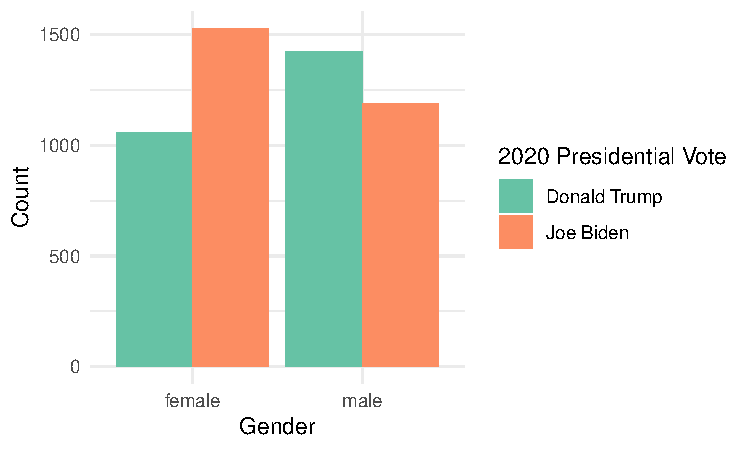
\includegraphics{2020-11-02-narrow-victory-for-biden-projected-in-2020-us-presidential-election_files/figure-latex/voteg1-1.pdf}
\caption{\label{fig:voteg1}2020 Presidential Votes by Gender}
\end{figure}

\begin{figure}
\centering
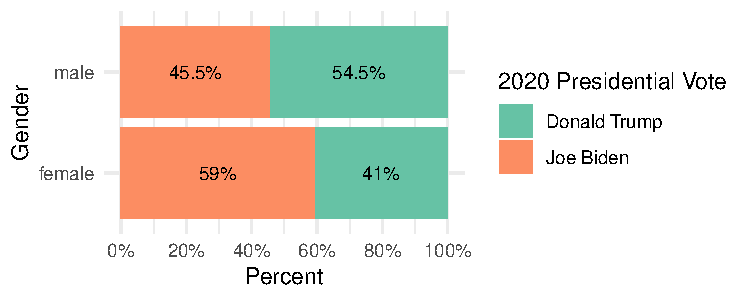
\includegraphics{2020-11-02-narrow-victory-for-biden-projected-in-2020-us-presidential-election_files/figure-latex/voteg2-1.pdf}
\caption{\label{fig:voteg2}2020 Presidential Vote Distribution by Gender}
\end{figure}

Regarding race, according to Figure 3 we can see that a large percentage of the respondents in the sample are white and appear to support Trump by a wide margin to Biden. However, in contrast, the Black/African American vote goes overwhelmingly to Biden (shown in Figure 4 with an overwhelming 76\% lead), whereas other racial categories are much more contested. It must be noted that in order to format this data for post-stratification with the ACS and ensure the subgroups that our eventual model would be enacted upon were big enough, several groups, such as Hawaiian, had to be conflated to the ``other asian or pacific islander'' category, justified as they were a small percentage of the population and their voting patterns tended to correlate. We nearly used whether a respondent was hispanic within the model, but in the end decided not to because the subcells were getting too small and we believed race in turn would suffice as a predictor regarding background.

\begin{figure}
\centering
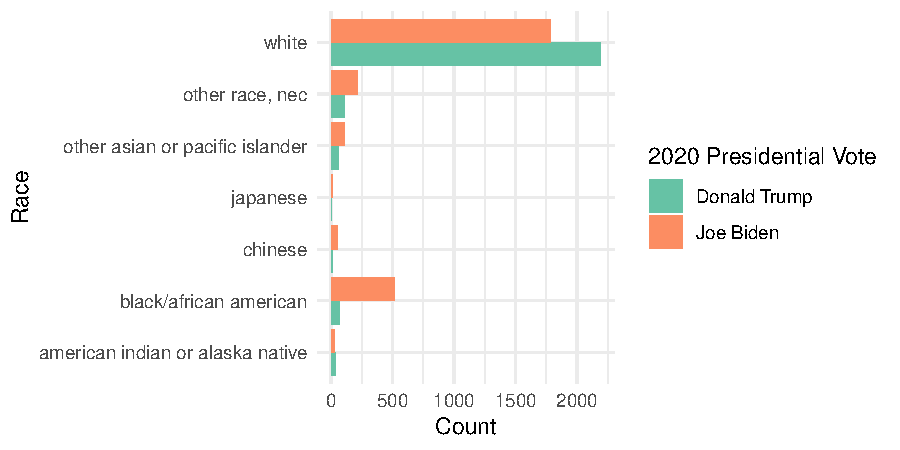
\includegraphics{2020-11-02-narrow-victory-for-biden-projected-in-2020-us-presidential-election_files/figure-latex/voter1-1.pdf}
\caption{\label{fig:voter1}2020 Presidential Votes by Race}
\end{figure}

\begin{figure}
\centering
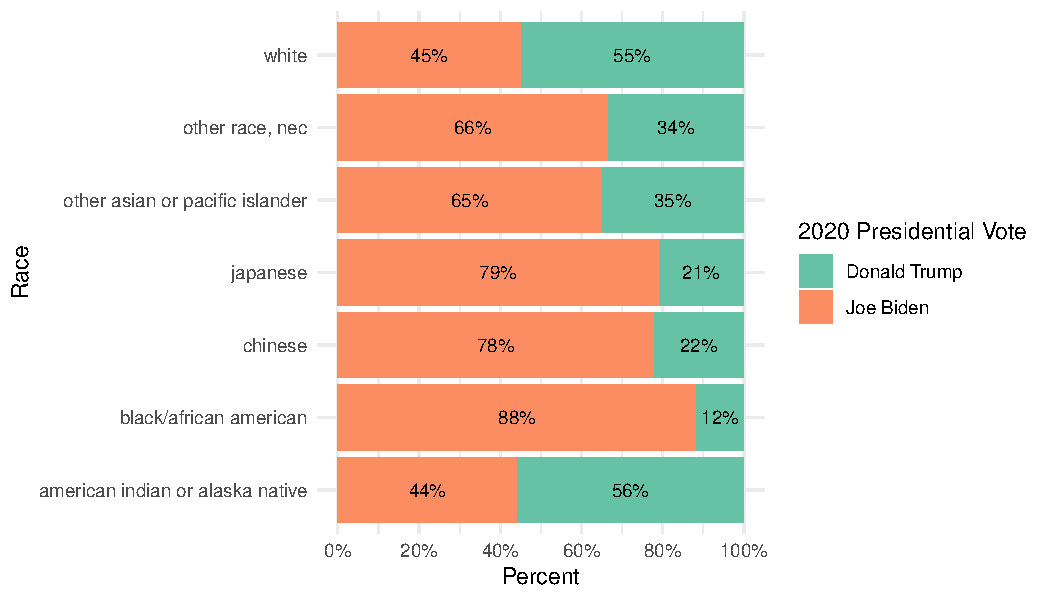
\includegraphics{2020-11-02-narrow-victory-for-biden-projected-in-2020-us-presidential-election_files/figure-latex/voter2-1.pdf}
\caption{\label{fig:voter2}2020 Presidential Vote Distribution by Race}
\end{figure}

For reasons due to ensuring that our subgroups remained large enough that there were a significant pool of samples for each, the education predictor was conflated to the categories: didn't graduate high school (from ``3rd Grade or less'', ``Middle School - Grades 4 - 8'' and ``Completed some high school''), graduated high school, didn't graduate college, and graduated college (from ``College Degree (such as B.A. or B.S.)'', ``Master's Degree'', ``Doctorate Degree'', ``Associate Degree'', ``Completed some graduate, but no degree''). This is because the combined subgroups tended to follow similar voting patterns and because given the small sizes of some of the variables in terms of observations, they did not affect the overall data significantly.

Figure 5 seems to demonstrate an overall trend that those who have graduated college tend to vote more for Biden than Trump, Figure 6 showing a 6.2\% difference. That being said, the other categories appear highly competitive, so perhaps education is not as strong a predictor as certain other variables mentioned earlier.

\begin{figure}
\centering
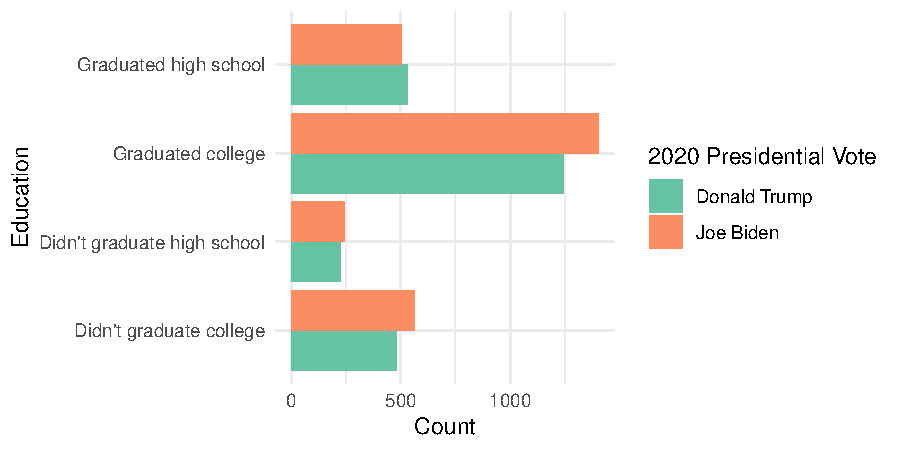
\includegraphics{2020-11-02-narrow-victory-for-biden-projected-in-2020-us-presidential-election_files/figure-latex/votee1-1.pdf}
\caption{\label{fig:votee1}2020 Presidential Votes by Education}
\end{figure}

\begin{figure}
\centering
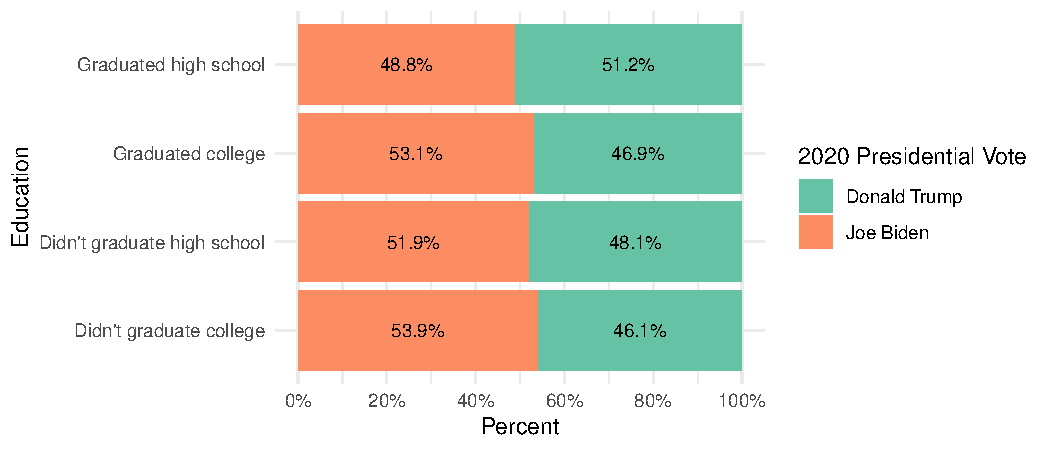
\includegraphics{2020-11-02-narrow-victory-for-biden-projected-in-2020-us-presidential-election_files/figure-latex/votee2-1.pdf}
\caption{\label{fig:votee2}2020 Presidential Vote Distribution by Education}
\end{figure}

\begin{figure}
\centering
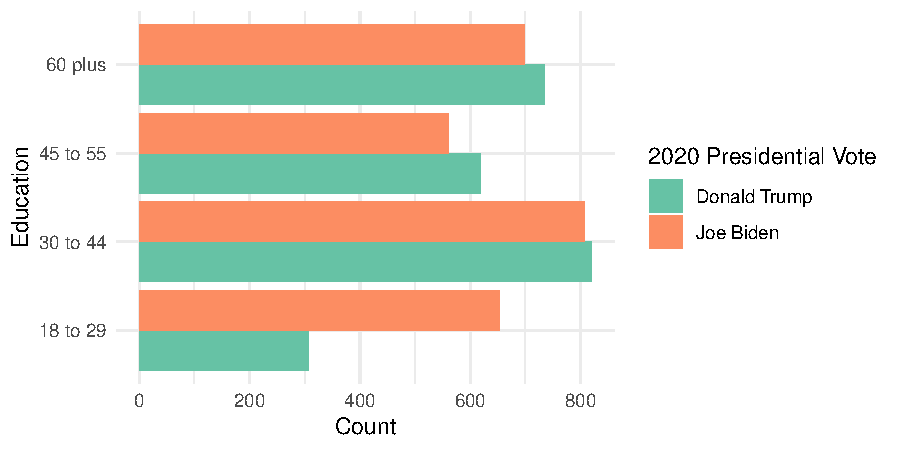
\includegraphics{2020-11-02-narrow-victory-for-biden-projected-in-2020-us-presidential-election_files/figure-latex/votea1-1.pdf}
\caption{\label{fig:votea1}2020 Presidential Votes by Age}
\end{figure}

According to Figure 7, it appears that Biden has a huge lead amongst young voters, and there is a direct correlation between the age group one belongs to and the likelihood that they'll vote for a candidate. For instance, Biden's lead is 36\% amongst voters 18 to 29 in Figure 8, very tightly tied with Trump for the age group 30 to 44, and appears to be somewhat behind Trump with older voters. This suggests age is an appropriate variable to gauge whether someone would vote for a particular candidate or not.

\begin{figure}
\centering
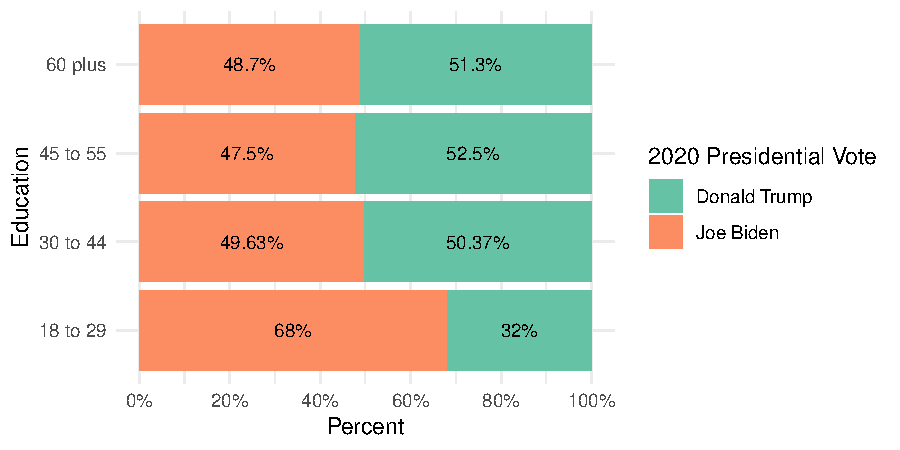
\includegraphics{2020-11-02-narrow-victory-for-biden-projected-in-2020-us-presidential-election_files/figure-latex/votea2-1.pdf}
\caption{\label{fig:votea2}2020 Presidential Vote Distribution by Age}
\end{figure}

America is divided into states, and the regional politics and situations within those states appears to play an important role, according to Figures 9 and 10, of which candidate that one would vote for. For instance, some states like California are 62\% skewed towards Biden out of decided voters, while others like Arizona are 68\% in favour of voting for Trump. Others like Wyoming are 50\% split exactly, so this shows that one's state has a hugely important influence/pressure on what candidate one is likely to vote for.

\begin{figure}
\centering
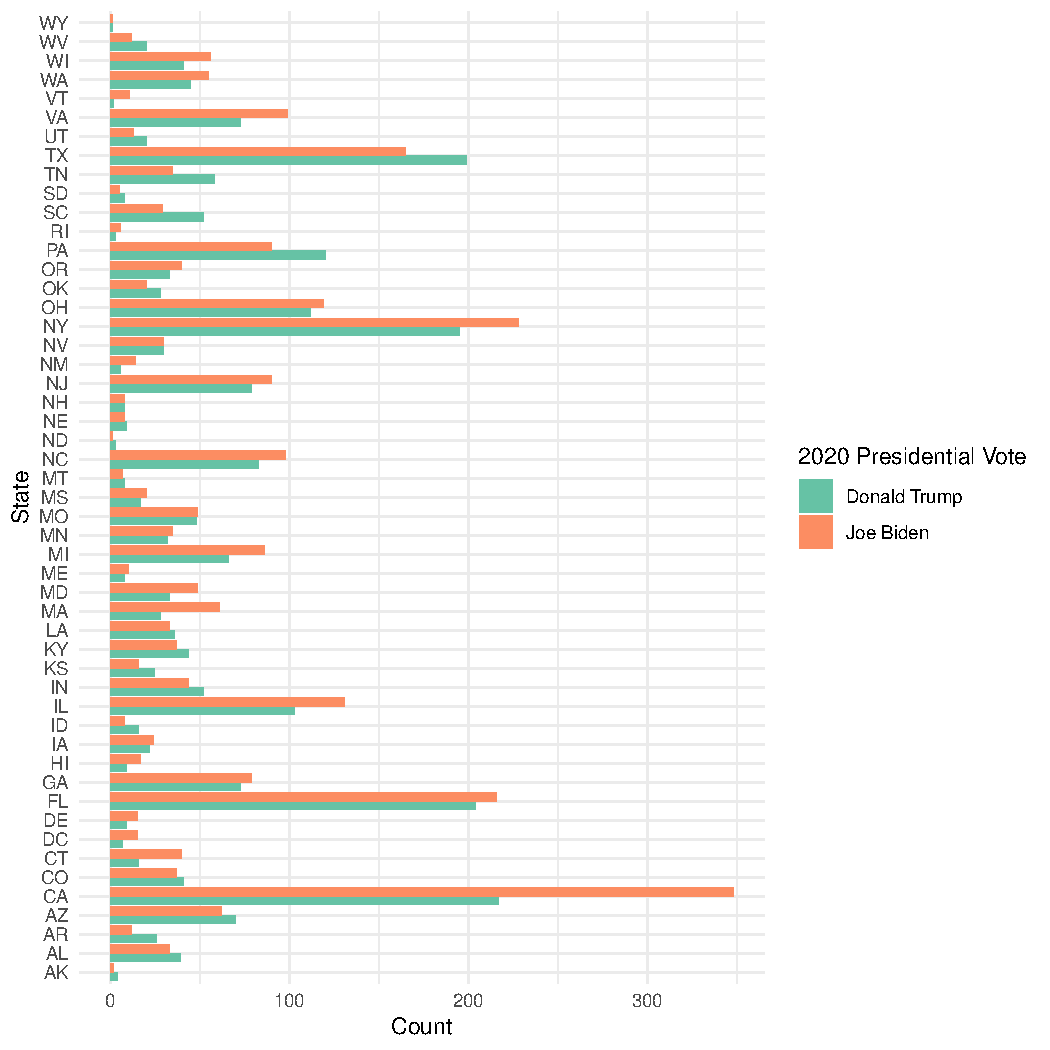
\includegraphics{2020-11-02-narrow-victory-for-biden-projected-in-2020-us-presidential-election_files/figure-latex/votes1-1.pdf}
\caption{\label{fig:votes1}2020 Presidential Votes by State}
\end{figure}

\begin{figure}
\centering
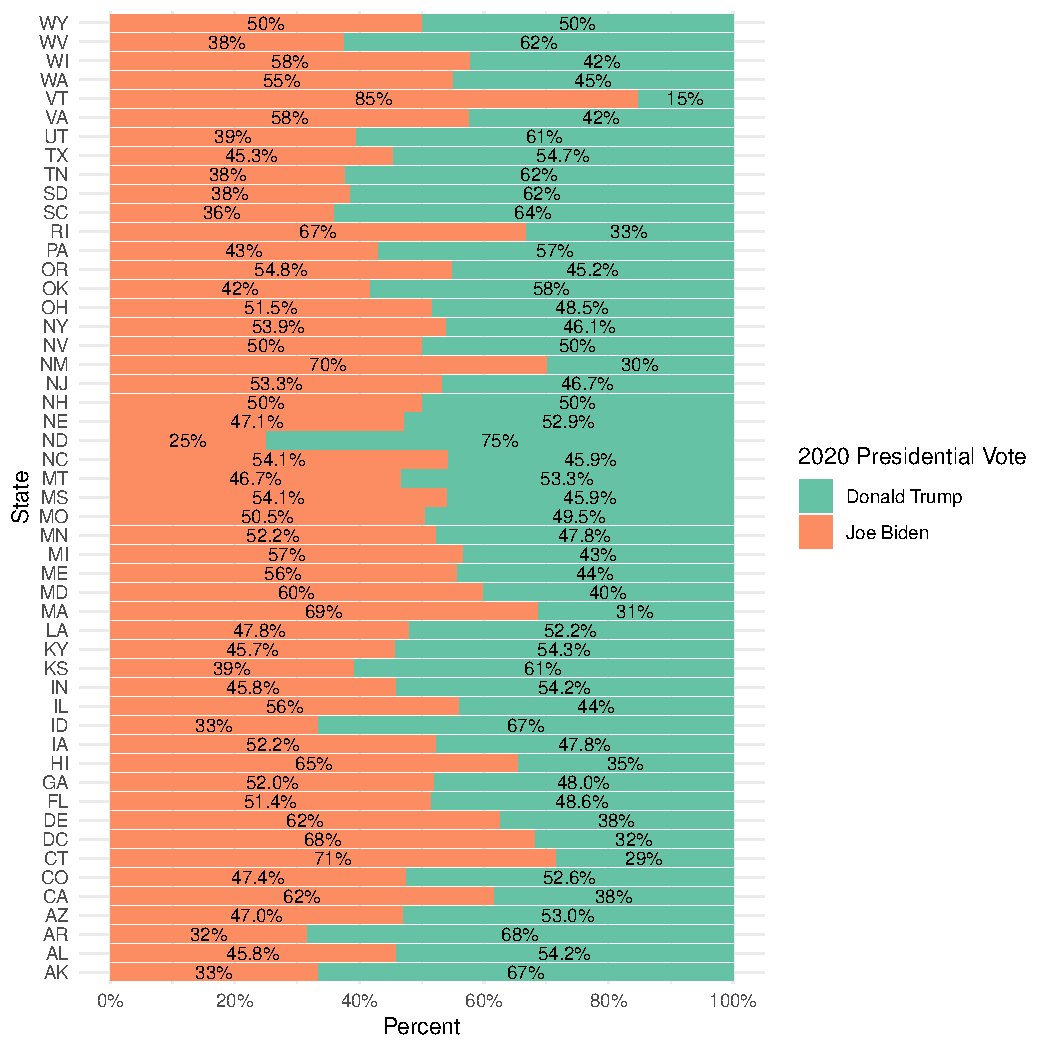
\includegraphics{2020-11-02-narrow-victory-for-biden-projected-in-2020-us-presidential-election_files/figure-latex/votes2-1.pdf}
\caption{\label{fig:votes2}2020 Presidential Vote Distribution by State}
\end{figure}

\hypertarget{post-stratification-data}{%
\subsection{Post-Stratification Data}\label{post-stratification-data}}

This data is offered by IPUMS, based on the American Community Surveys from the U.S. Census Bureau. In this project, we use the data collected from the American Community Survey 2018 \citep{citeIPUMS}.

The target population in this case is every resident in the United States (not necessarily every voter in the United States, something we kept in mind when we engaged in the process of data-cleaning through taking out underage respondents who cannot vote, for instance). The sampling population is all the living quarters in the United States (in which both housing units and group quarters, such as college residence halls, military barracks, faculties for the homeless, correctional facilities, group homes, nursing facilities and more, are considered ``living quarters''), and thus the sampling frame is the list of living quarters that were picked out from the sampling population.

There are two phases of determining the samples for housing units: in the first, new samples are selected (in September/October of the previous year), and in the second, non-responding addresses are selected for personal interviewing (in January of the current year). This removes the percentage of non-respondents. These samples are selected from the sampling population, found via the US Census Bureau's ``Master Address File'', which has a list of all living quarters and certain non-residential buildings \citep{citeACS}.

For group quarters, certain exclusions are applied for privacy and feasibility reasons (ex. domestic violence shelters, dangerous encampments and more). Field representatives do interviews of qualifying group quarters, in which people are organized into groups of 10 \citep{citeACS}.

For housing units, data collection is done through Internet, mail, telephone and personal visit. This includes emailing respondents or offering paper questionnaires for ease of accessibility. In the case of non-response, there is a follow-up with a computer-assisted telephone interview. This data collection is made further accessible with language assistance, such as translated resources and interviewers that can speak several languages through telephone contact \citep{citeACS}.

This methodology has several pros and cons---in terms of pros, a lot of care has been taken to lower the level of non-response. Not only through computer-assisted interviewing in order to follow up with those who do not respond, but this survey also takes into account group quarters for those who may not have access to a residential home. This ensures that the underprivileged are not overlooked in the survey. Because of the care taken to make sure those not proficient in English can access the survey, there will be greater representation of the less dominant culture given America is primarily an English-speaking country. The second stage, which involves contacting people once again who didn't respond the first time, offers even more accuracy. However, this does not guarantee complete response in the least, and this data is accurate to 2018. The population distribution may have changed since then and the data could be outdated to the current demographics. Moreover, this dataset asks for the respondents' sex rather than their gender, providing then ignoring the demographic of non-cisgender and gender non-conforming people in their methodology \citep{citeACS}.

As mentioned in the previous section, the variables at play are the state, the gender (taken from the sex and assumed to the same), age, race and education level of the respondant. Variables that were created for the sake of post-stratification are the number of cases under each combination of the five variables (so the size of the cell), and the proportion of each cell with regard to the total population \citep{citeACS}.

Like with the previous dataset for the survey, this one had to combine race into particular categories. In this one, observations such as ``Two major races'' had to be combined into ``Other race, nec'' as it was the most accurate category. Education was split into the same categories mentioned earlier, associate degrees and such all folded under college degree for the sake of simplicity.

Below are some distributions of the variables of interest.

\begin{figure}
\centering
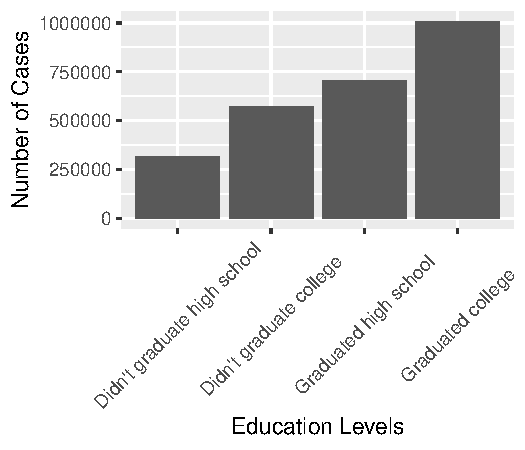
\includegraphics{2020-11-02-narrow-victory-for-biden-projected-in-2020-us-presidential-election_files/figure-latex/educd-1.pdf}
\caption{\label{fig:educd}Distribution of Education}
\end{figure}

\begin{figure}
\centering
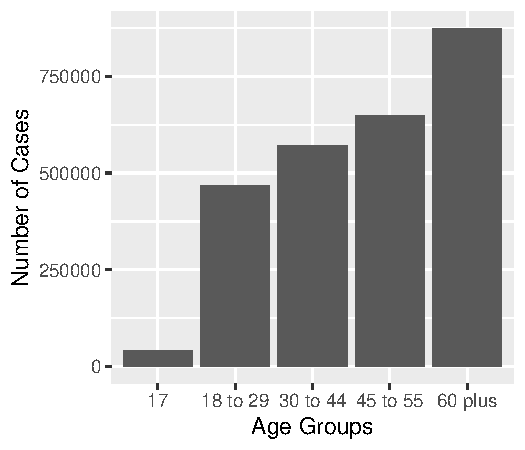
\includegraphics{2020-11-02-narrow-victory-for-biden-projected-in-2020-us-presidential-election_files/figure-latex/age-1.pdf}
\caption{\label{fig:age}Distribution of Age}
\end{figure}

As we can identify in Figure 11, there are more people who have graduated from college than simply high school. Moreover, there are more people who didn't graduate from college than didn't graduate high school. Thus, a sizable proportion of the US electorate is relatively educated. In Figure 12, people who are 60+ are by far the largest age group, showing an aging population. Given that this population tends to support Trump, this is an important statistic to keep an eye on.

You can see from Table 1 that the total number of people who completed high school is 65.83\% of the overall population, whereas the proportion of people who completed college is 38.75\%. Based on Table 2, the people whose age are 60 and above has 35.4\% of overall population, which is the largest portion in US.

\begin{figure}
\centering
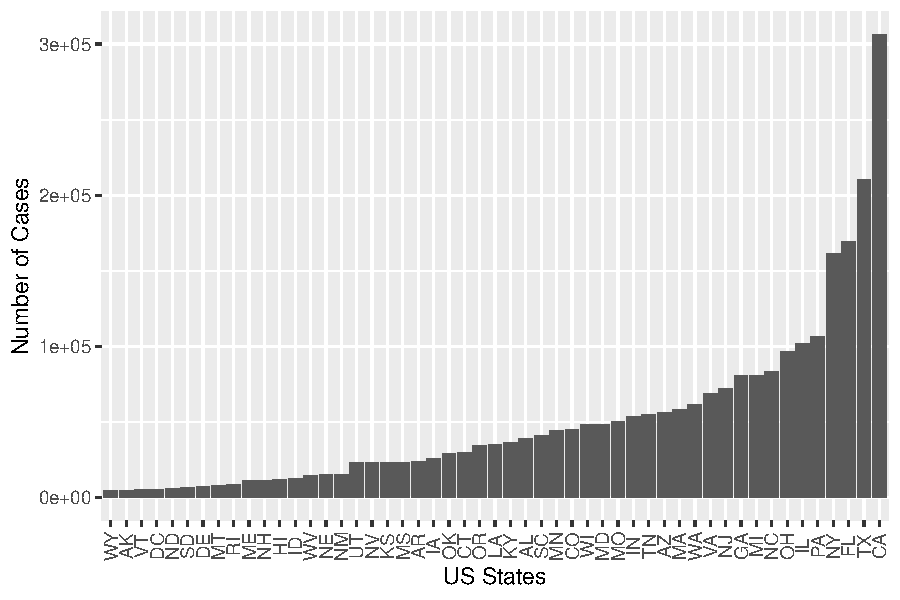
\includegraphics{2020-11-02-narrow-victory-for-biden-projected-in-2020-us-presidential-election_files/figure-latex/state-1.pdf}
\caption{\label{fig:state}Population for Each State}
\end{figure}

\begin{figure}
\centering
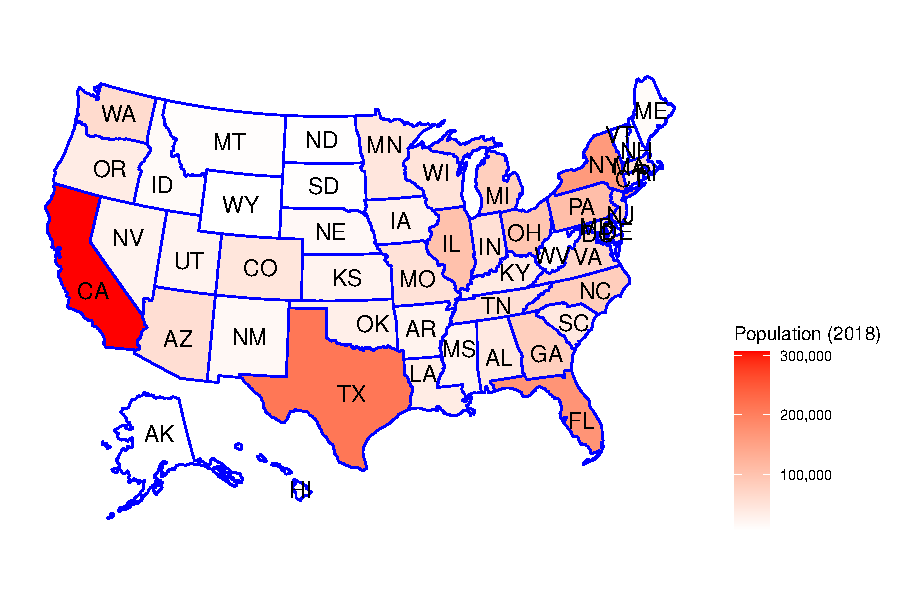
\includegraphics{2020-11-02-narrow-victory-for-biden-projected-in-2020-us-presidential-election_files/figure-latex/state1-1.pdf}
\caption{\label{fig:state1}States Population Map}
\end{figure}

Figure 13 shows the distribution of population amongst US states. The largest by far is California (shown earlier to skew towards Biden), the second largest Texas (which tends to skew towards Trump). Figure 14 shows that the population is highest amongst coastal and southern states, and this may skew the popular vote from the electoral vote.

\begin{figure}
\centering
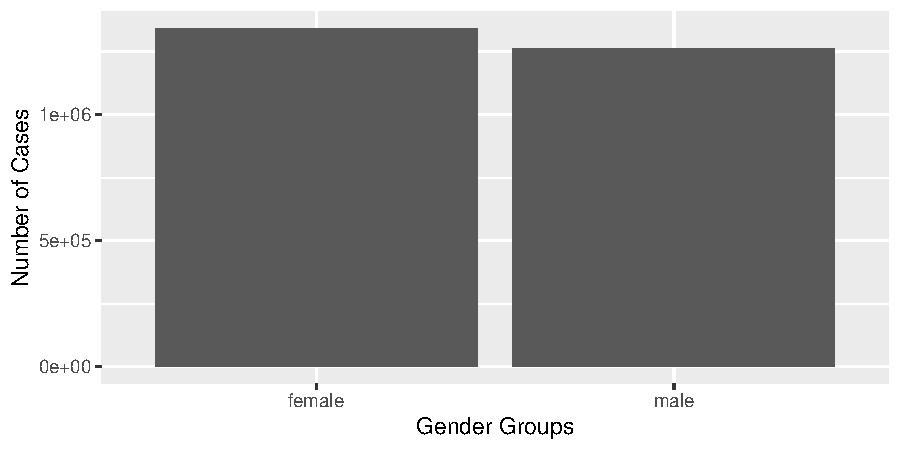
\includegraphics{2020-11-02-narrow-victory-for-biden-projected-in-2020-us-presidential-election_files/figure-latex/gender-1.pdf}
\caption{\label{fig:gender}Distribution of Gender}
\end{figure}

\begin{figure}
\centering
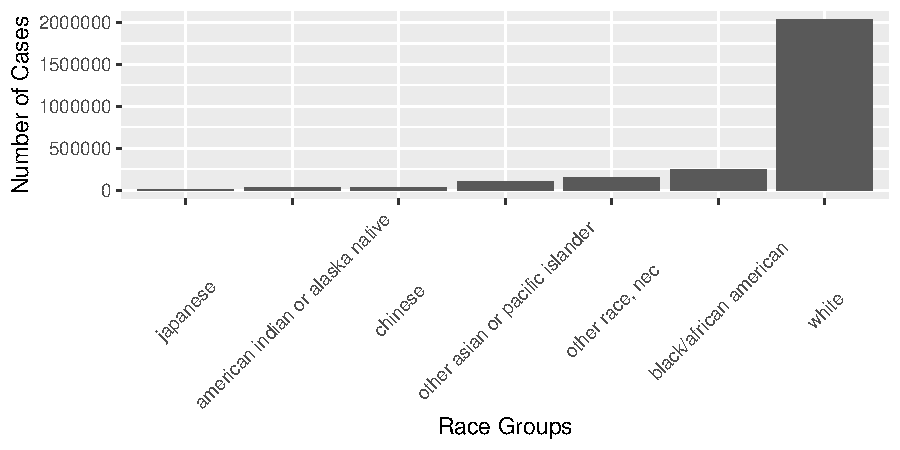
\includegraphics{2020-11-02-narrow-victory-for-biden-projected-in-2020-us-presidential-election_files/figure-latex/race-1.pdf}
\caption{\label{fig:race}Population for Races}
\end{figure}

Figure 15 has the distribution of gender, shown to be 51.56\% for women and 48.44\% for men.
Figure 16 shows that much like the survey data from \citet{citeSurvey}, the largest race group in the US is white, and the second largest race group is Black/African American. Based on Table 4, the white population has 2,031,750 people, and 78.05\% of the overall population. The Black/African American population has 249,642 people, and 9.59\% of the overall population. This indicates they are important sectors of the population for the candidates to campaign for.

\#Modeling with MRP

Different levels of the variables of interest in the post-stratification process show different responses for presidential votes (support for Joe Biden). The survey's demographics differ from the actual population, therefore certain groups of individuals were under/overrepresented in the survey, leading to sampling bias. Therefore, we use the survey sample data to infer presidential votes on the census population in the US using post-stratification variables.
In order to address the over/underrepresentation of certain demographics within the survey results, we perform multilevel regression and poststratification (MRP) on the survey data from the Democracy Fund Voter Study Group with census data from the ACS provided by IPUMS. In doing so, we calculate the proportions of each group of individuals from the actual population distribution, the census data, and apply the results of the survey onto these proportions. In doing so, we basically reweigh the results from the survey to post-stratify our results to produce an estimate of the 2020 US election that more accurately represents the actual population distribution. This method is effective for using non-representative samples to make predictions, however can be quite troublesome when cells created of each group are too small, creating unstable results for each variable \citep{citeMJAlexander}. Throughout our cleaning process, we had to alter the way each group was levelled off in order to create cells that were large enough to produce stable results.

\textbf{Steps of MRP}

\begin{enumerate}
\def\labelenumi{\arabic{enumi}.}
\tightlist
\item
  Gather sample data(survey data) with certain key variables in mind (state, age, gender, education, race).
\item
  Gather population data(census data) with the same key variables.
\item
  Match the variables of each dataset so each of the cells will correspond with each other, if necessary.
\item
  Decide the quantity you would like to measure in the sample (support for Joe Biden = 1, support for Donald Trump = 0).
\item
  Estimate quantity of interest in the population using MRP to predict using the key demographics from the sample.
\item
  Apply this model to the new data (census data) and make estimates of predictions for the population.
\end{enumerate}

Our first approach in modelling predictions was to look at linear regression on the \emph{dummy\_vote} variable and the five explanatory variables selected using the function \emph{lm()}. We chose to use a frequentist approach, where parameters of interest are fixed, first to explore both datasets. There are assumptions made about the data when choosing to perform ordinary linear regression on the survey data .
1. The relationship between all explanatory variables and the response variable follows a linear pattern.
2. The variance of the residuals is constant for all values/levels of the explanatory variables.
3. Observations are independent of each other.
4. All variables are normally distributed.
The estimates for the linear regression model and the generalized logistic regression model provide the same estimates for the explanatory variables, in our case, the proportion of votes for Mr.~Joe Biden, however, the variances for each explanatory variable will differ.

Linear regression general formula:
\[ y = \beta_0 + \beta_1x_1 + \epsilon \]

Since the outcome of the response variable is either 1 or 0 (1 indicating a vote for Joe Biden), a logistic regression can be used to address the binary response variable \citep{citeAndrew}. The function \emph{glm} from the allows defining of the response variable to a binomial distribution to the logistic regression. For p as the probability of support for Joe Biden, the logistic regression can be modelled in this formula:

\[ \log(\frac{p}{1-p}) = \beta_0 + \beta_2x_2 + ... + \beta_kx_k\]

The coefficients in this logistic regression model represent the change in log odds of support for Joe Biden. Since gender was only recorded as either `male' or `female, this explanatory variable is binary. Race, education, state and age group were all categorical variables
By conducting logistic regression on the multiple explanatory variables with multiple levels, a few things jumped out. Since many variables and cells are being represented in the model, we wanted to find out which explanatory variables were statistically important to the raw data obtained from the sample in order to find the best fitting models for predicting on other populations. Certain variables could be identified as statistically important by evaluating the p-values for each, and the estimate for each coefficient.
Our second approach in modelling predictions was to fit a Bayesian model to address the fact that we are predicting a variable in the census data based on the survey data. In using a Bayesian model, we intended to compare our prediction results with a frequentist model to compare how much the prediction was influenced by the census proportions. We used the \emph{brm} function from the \textbf{brms} package \citep[\citet{citerstan}]{citebrms} and organized the data and results with the \textbf{tidybayes} \citep{citetidybayes} ,\textbf{tidyverse} \citep{citetidyverse}, \textbf{magrittr} \citep{citemagrittr}, \textbf{gridExtra} \citep{citegridExtra}, usmap \citep{citeusmap}, \textbf{scales} \citep{citescales}, \textbf{haven} \citep{citehaven}, \textbf{broom} \citep{citebroom} and \textbf{here} \citep{citehere} packages. Bayesian inference assumes certain priors about the parameters of interest, meaning that the parameters are not fixed, rather they follow some type of distribution \citep{citePChristianBurkner}. Since our parameter of interest is being formed in the post-stratification data, our new parameter of interest is the proportion of Biden support in the census population, which also has a random binary outcome. In the Bayesian model, we assume a bernoulli distribution for the support of Joe Biden in the US 2020 election.

Bayes' Rule: \[ P(A|B) = \frac{P(B|A)P(A)}{P(A)} \]

A is the prior distribution that is assumed about the parameter of interest, in our case the distribution of the proportion of Biden support in the census data whereas B is the census data \citep{citeDSimpson}.

Bernoulli Distribution:
\[ f(k;p) = \begin{cases} p & \text{if k$ = 1$}, \\ 1- p & \text{if k = 0}. \end{cases} \]

There are two main things to look out in this comparison of estimates based on the raw data and the MRP: how the post-stratification changes the estimate obtained from the raw data, and how much variance each estimate has based on each level of the variable. In addition, analyzing the proportion of the census data and the survey data will provide additional insight on how the census proportions of groups affect the MRP estimate. As shown in Figure 19, where the estimates based on each State are being compared, the MRP estimate does not differ significantly from the raw data. This indicates that the proportion of individuals surveyed residing in each state was similar to what was observed within the census data. The red bars indicate the 97.5\% confidence interval for each estimate.

\#Results

\begin{figure}
\centering
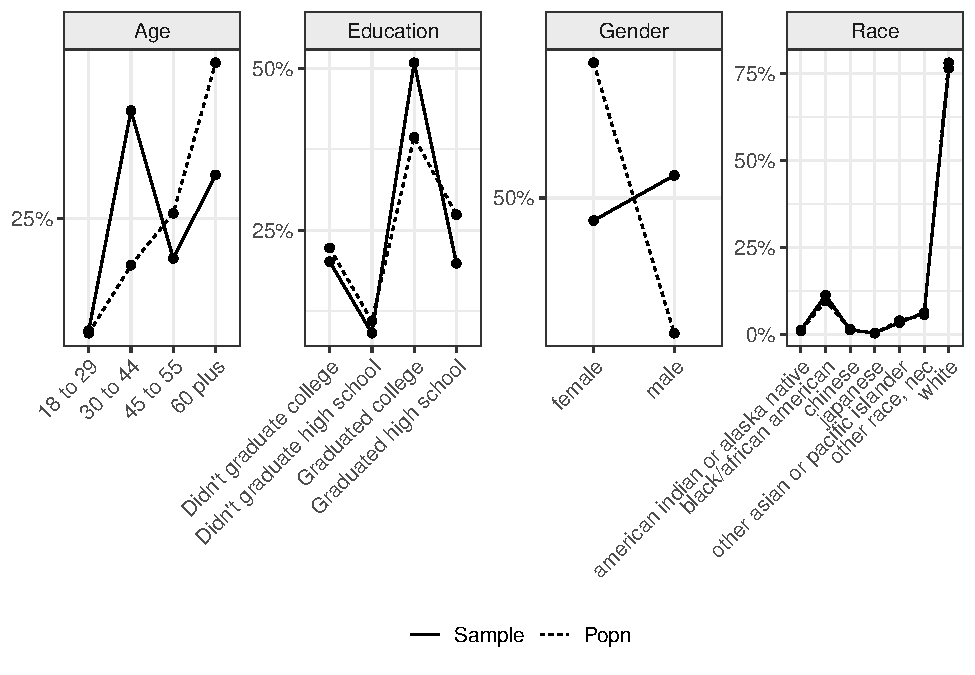
\includegraphics{2020-11-02-narrow-victory-for-biden-projected-in-2020-us-presidential-election_files/figure-latex/popplots-1.pdf}
\caption{\label{fig:popplots}Demographic Proportions}
\end{figure}

\begin{figure}
\centering
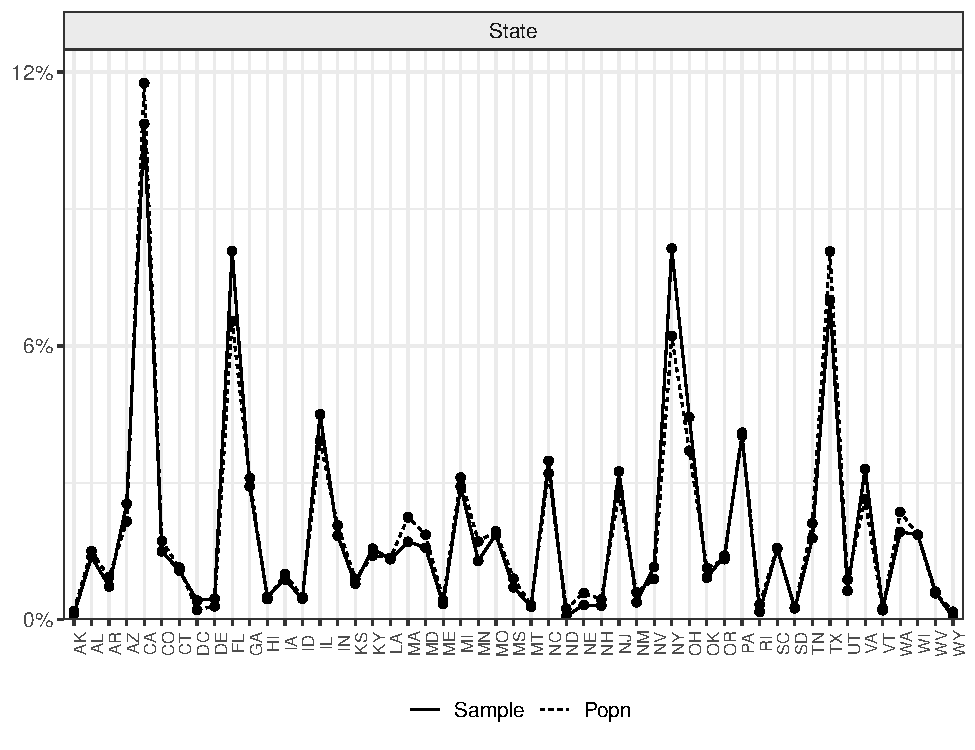
\includegraphics{2020-11-02-narrow-victory-for-biden-projected-in-2020-us-presidential-election_files/figure-latex/popplots1-1.pdf}
\caption{\label{fig:popplots1}Proportions by State}
\end{figure}

\hypertarget{bayesian-approach-to-mrp}{%
\subsection{Bayesian Approach to MRP}\label{bayesian-approach-to-mrp}}

Figures 19-23 are graph the distibution of estimates using Bayesian inference in the \textbf{brms} package \citep{citebrms}.

\begin{figure}
\centering
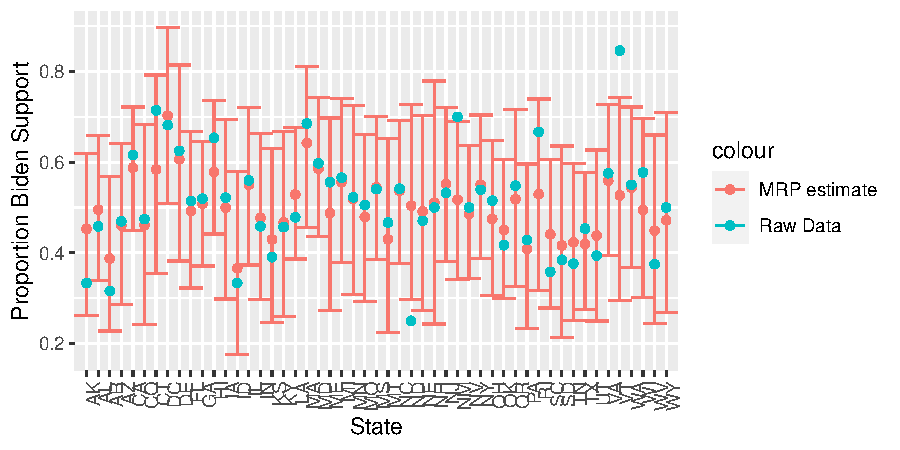
\includegraphics{2020-11-02-narrow-victory-for-biden-projected-in-2020-us-presidential-election_files/figure-latex/bayesplot-1.pdf}
\caption{\label{fig:bayesplot}Comparing Survey Estimates with MRP Estimates by State}
\end{figure}

The prediction of proportion of support for Biden in the post-stratification across each state shown in Figure 19 does not seem to differ much from the original proportions found in the sample distribution, considering that each state has relatively the same amount of proportions across both datasets, this is not surprising. However, there were a few states that had quite different estimates. Vermount, Rhode Island and New Mexico were estimated to be less supportive of Joe Biden in the MRP modelling whereas Alaska and North Dakota were more supportive of Joe Biden than in the original raw sampling data.

\begin{figure}
\centering
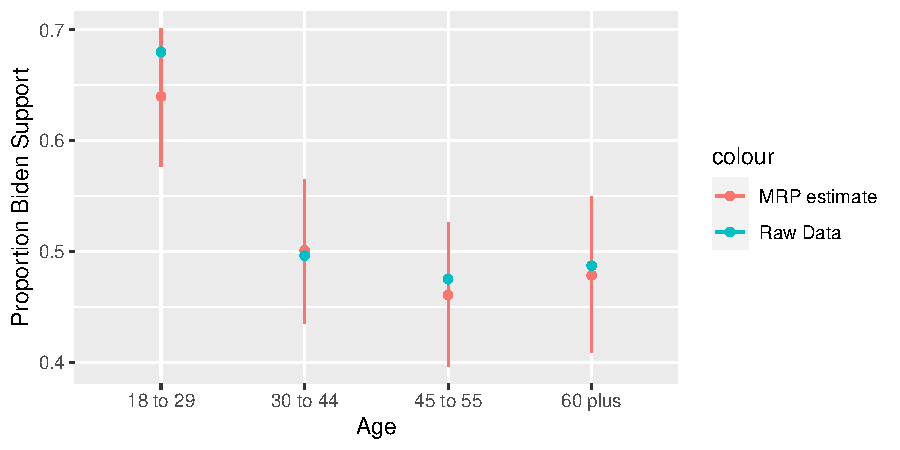
\includegraphics{2020-11-02-narrow-victory-for-biden-projected-in-2020-us-presidential-election_files/figure-latex/bayesplot1-1.pdf}
\caption{\label{fig:bayesplot1}Comparing Survey Estimates with MRP Estimates by Age}
\end{figure}

The estimate for the Biden support for individuals in age group 18-19 were slightly higher in the raw data shown in Figure 20. However, this age group was still particularly in high favor of Joe Biden as both estimates were over 60\%. Individuals in the 30-45 age category seemed to respond more to the polling survey, thus creating slightly biased results. However, the estimates for individuals in the 30-45 age category were consistent in the post-stratification data and the survey data. It appears that among both groups, older age groups appear to be less supportive of Joe Biden, but only marginally.

\begin{figure}
\centering
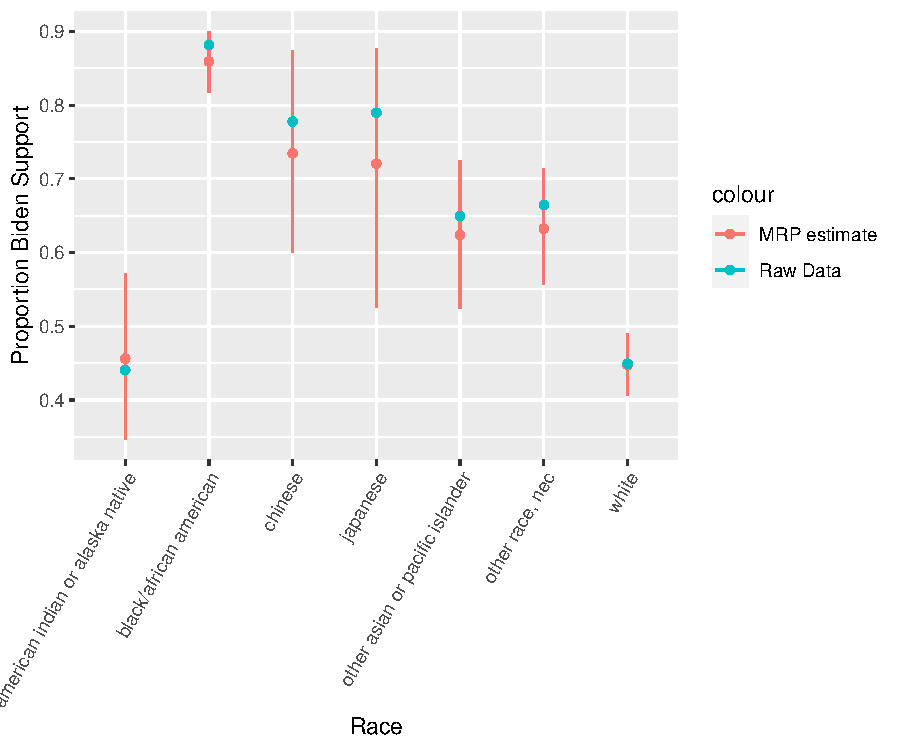
\includegraphics{2020-11-02-narrow-victory-for-biden-projected-in-2020-us-presidential-election_files/figure-latex/bayesplot2-1.pdf}
\caption{\label{fig:bayesplot2}Comparing Survey Estimates with MRP Estimates by Race}
\end{figure}

Estimates between survey data and post-stratification data remain relatively the same for race shwon in Figure 21. Among black/African Americans, Chinese and Japanese age groups, Biden appears to be well supported with estimates exceeding 70\% for each age group. American Indian and Alaska Natives as well as white individuals were slightly less supportive. Based on this graph alone it would appear that Joe Biden would have a significant lead, however, the proportion of white individuals in the census population and the survey population exceeds 75\%, comprising a significant portion of the population.

\begin{figure}
\centering
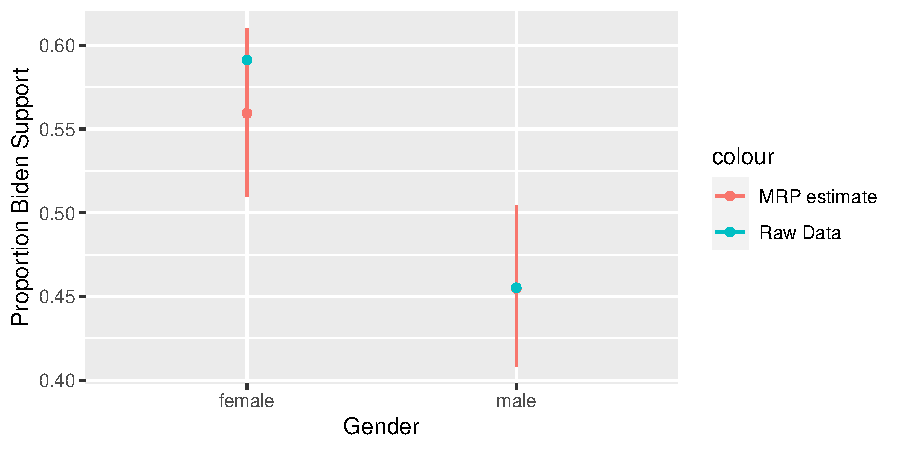
\includegraphics{2020-11-02-narrow-victory-for-biden-projected-in-2020-us-presidential-election_files/figure-latex/bayesplot3-1.pdf}
\caption{\label{fig:bayesplot3}Comparing Survey Estimates with MRP Estimates by Gender}
\end{figure}

On average, females tend to be more supportive of Joe Biden while males tend to support Donald Trump as shwon in Figure 22. Although females represent more of the census population than males, this is not reflected in the survey where males had a slightly higher response rate. This is reflected in the difference between estimates of females being decreased in the MRP estimate by almost 5\%.

\begin{figure}
\centering
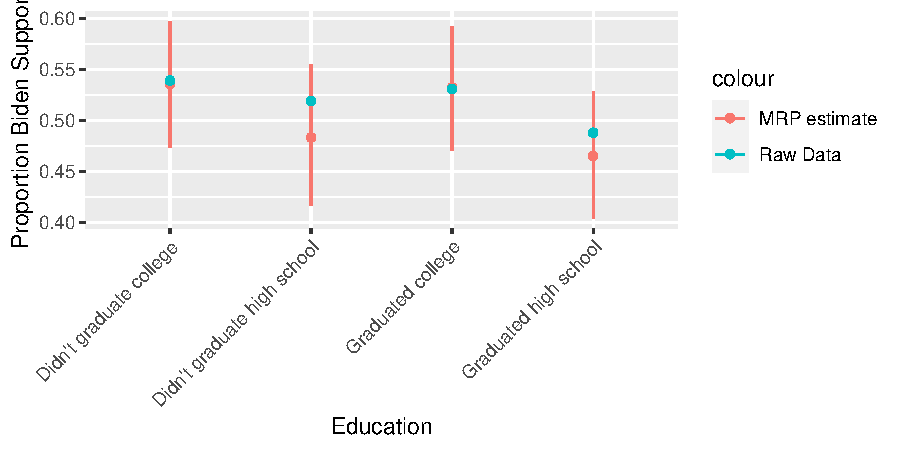
\includegraphics{2020-11-02-narrow-victory-for-biden-projected-in-2020-us-presidential-election_files/figure-latex/bayesplot4-1.pdf}
\caption{\label{fig:bayesplot4}Comparing Survey Estimates with MRP Estimates by Education}
\end{figure}

It appears that there is an overrepresentation of individuals who have graduated college who responded to the surveys reflected in Figure 23. In addition, there is an underrepresentation of those who had just graduated high school. The MRP estimate was lower than the raw data for both individuals who graduated high school and who did not graduate high school.

\hypertarget{discussion}{%
\section{Discussion}\label{discussion}}

Information of interest collected through surveys is often not representative of the population that we are looking into. Due to the nature of traditional surveys, accurately representing the actual population of interest is difficult, expensive, timely and perhaps impossible when dealing with very large-scaled populations. Luckily, there are some ways to address this issue by using MRP to correct misproportions in samplings. Survey data collected from the Democracy Fund Voter Study Group employed stratified sampling. Stratified sampling divides the population into subpopulations based on certain characteristics or attributes. These subpopulations are called strata. Stratified sampling helps to somewhat control the proportions of certains groups being included in the sample instead of having all groups of individuals having an equal chance to be represented in the survey. Thus the sampling data is very extensive and somewhat pre-weighted due to stratified sampling, however, looking at the differences in proportions between each group there still exists some sampling biases for certain groups, such as age. Indicated in the logistic regression, certain factors such as age, gender and race had lower p-values, indicating they were more statistically important to the model than variables such as state. Only certain states reported low p-values, such as Connecticut, Massachusetts and Vermont, indicating statistical importance on the logistical model.
In the logistic regression and Bayesian model, we found that Biden had a predicted vote proportion of 50.1\% and 51.03\%, respectively . Considering that the proportions of all the levels of variables did not differ greatly, except across age groups, the predictions remained relatively similar to each other. The survey data was already pre-weighted to a certain extent using stratified sampling, therefore proportions across race for each of the datasets were very similar. The main difference between proportions in the datasets was within the age group, where younger individuals tended not to respond to surveys as much as middle-aged individuals. The MRP estimates that were quite different from the raw data for each state were moste likely affected by the different age groups sampled and possibly even gender. We must also not forget about particular cells to identify any cross sectional relevance of the variables and if there is any type of relationship for certain groups. Conducting MRP over 5 variables of interest helped to identify and narrow down key variables and levels that could further influence voting choice in the US 2020 elections.

It is worthwhile to mention that the survey used was collected back in June. Since then, many events surrounding the election have changed public opinion of both candidates, and therefore will ultimately affect the final outcome of the US 2020 Presidential Election taking place on November 3rd, 2020. Further work might look into conducting bayesian inference models across time to model changes over periods of time leading up to the election to provide further insight. Time series analysis can be helpful in understanding trends that are relative to the election date.

MRP can be used as a tool when a population of interest is identified with key variables that can affect the variable of interest, which can be matched to a sample population to formulate inferences. Comparing the sample estimate of Joe Biden support with the forecasted estimates on the census population provides further tools for research to explore nuances in the data and additional differences. MRP ultimately can identify certain variables of interest as predictions to perform smaller scaled polling to include more levels of variables of the data that were hidden in the way we categorized individuals within each of the groups, such as race and education in our case. It is relatively quick, easy and cost effective to perform on data given a survey with matching key variables with a more representative population.

MRP has lead many studies to significant and representative models on actual populations from samples, however it does not come without flaws. Insufficient estimates can be caused by lack of some demographic predictors, insufficient data from surveying as well as lack of regularization. In some cases, selecting certain variables as predictors lead to extremely small cell counts for certain groups, therefore producing unstable estimations. Through our cleaning process of both datasets, some tweaking of the variables and levels had to be made in order to match all variables to perform MRP. The sample data was extremely extensive and all-inclusive of any possible variable, however this is not always the case. The way that information demographic variables and in the sample and census data are sometimes collected and recorded in different forms. \citep{citeLKennedy} \citep{citeAGelman}.

\hypertarget{appendix}{%
\section{Appendix:}\label{appendix}}

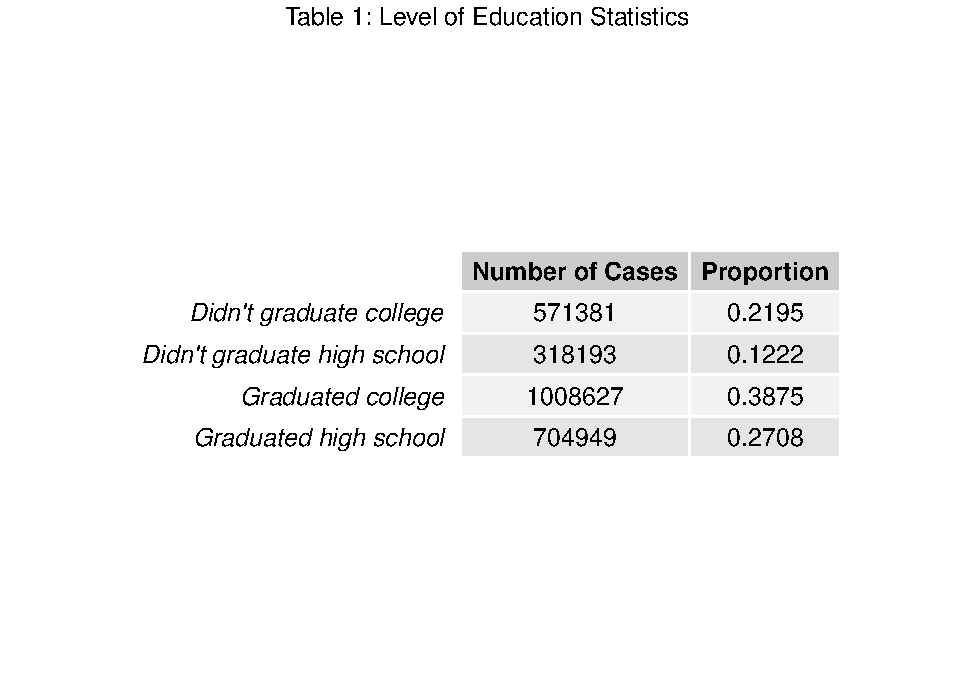
\includegraphics{2020-11-02-narrow-victory-for-biden-projected-in-2020-us-presidential-election_files/figure-latex/appendix-1.pdf} 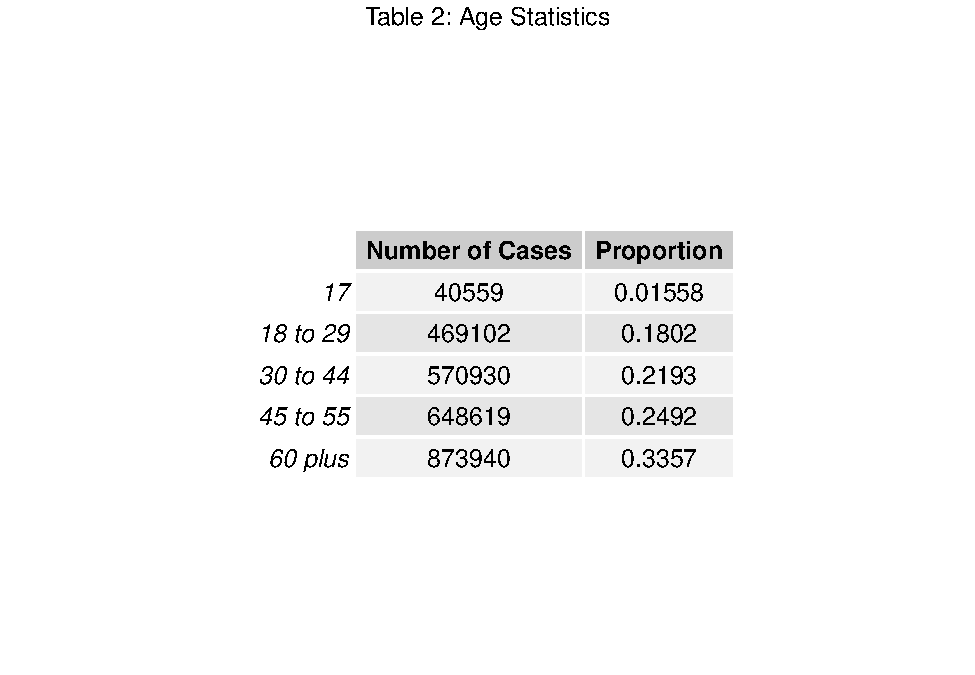
\includegraphics{2020-11-02-narrow-victory-for-biden-projected-in-2020-us-presidential-election_files/figure-latex/appendix-2.pdf} 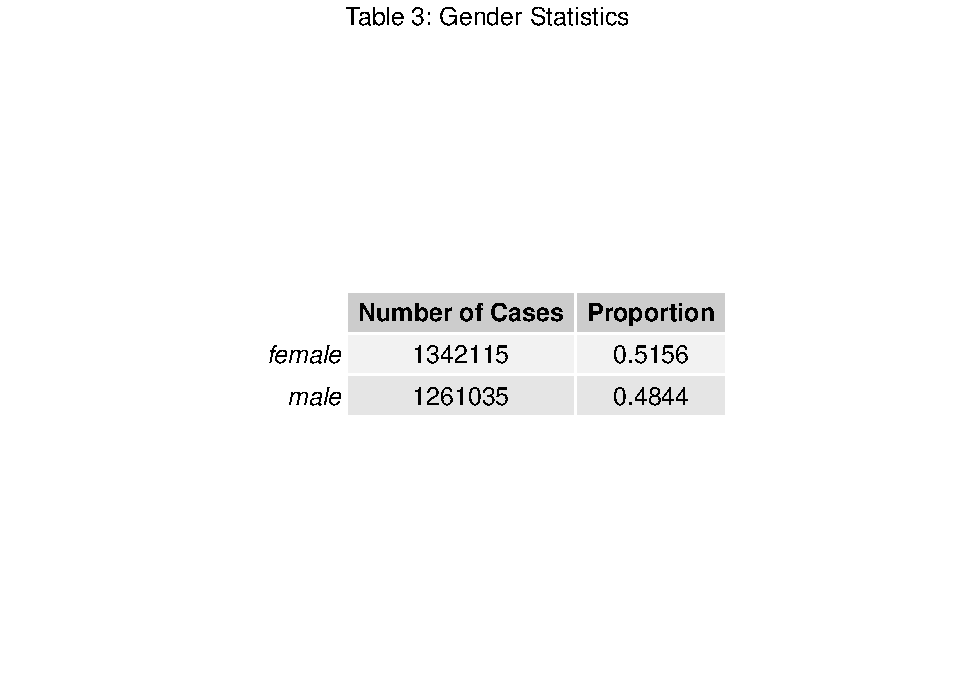
\includegraphics{2020-11-02-narrow-victory-for-biden-projected-in-2020-us-presidential-election_files/figure-latex/appendix-3.pdf} 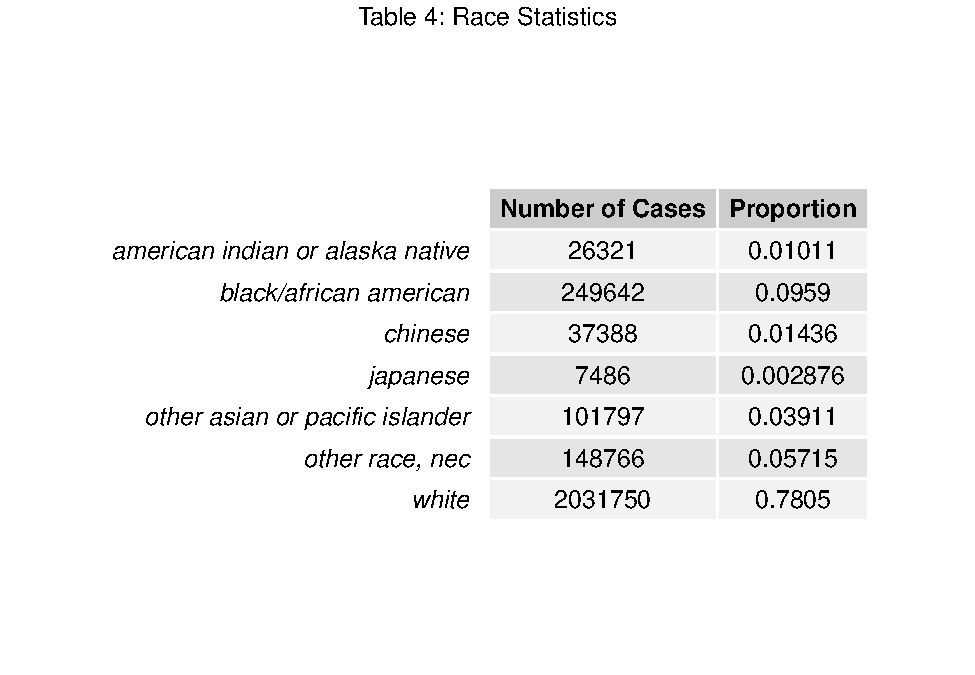
\includegraphics{2020-11-02-narrow-victory-for-biden-projected-in-2020-us-presidential-election_files/figure-latex/appendix-4.pdf}

  \bibliography{references.bib}

\end{document}
